% Options for packages loaded elsewhere
\PassOptionsToPackage{unicode}{hyperref}
\PassOptionsToPackage{hyphens}{url}
\PassOptionsToPackage{dvipsnames,svgnames,x11names}{xcolor}
%
\documentclass[
  14,
  a4paper,
  DIV=11,
  numbers=noendperiod]{scrartcl}

\usepackage{amsmath,amssymb}
\usepackage{iftex}
\ifPDFTeX
  \usepackage[T1]{fontenc}
  \usepackage[utf8]{inputenc}
  \usepackage{textcomp} % provide euro and other symbols
\else % if luatex or xetex
  \usepackage{unicode-math}
  \defaultfontfeatures{Scale=MatchLowercase}
  \defaultfontfeatures[\rmfamily]{Ligatures=TeX,Scale=1}
\fi
\usepackage{lmodern}
\ifPDFTeX\else  
    % xetex/luatex font selection
  \setmainfont[]{Arial}
  \setsansfont[]{Arial}
  \setmonofont[Scale=0.85]{Courier New}
\fi
% Use upquote if available, for straight quotes in verbatim environments
\IfFileExists{upquote.sty}{\usepackage{upquote}}{}
\IfFileExists{microtype.sty}{% use microtype if available
  \usepackage[]{microtype}
  \UseMicrotypeSet[protrusion]{basicmath} % disable protrusion for tt fonts
}{}
\makeatletter
\@ifundefined{KOMAClassName}{% if non-KOMA class
  \IfFileExists{parskip.sty}{%
    \usepackage{parskip}
  }{% else
    \setlength{\parindent}{0pt}
    \setlength{\parskip}{6pt plus 2pt minus 1pt}}
}{% if KOMA class
  \KOMAoptions{parskip=half}}
\makeatother
\usepackage{xcolor}
\setlength{\emergencystretch}{3em} % prevent overfull lines
\setcounter{secnumdepth}{-\maxdimen} % remove section numbering
% Make \paragraph and \subparagraph free-standing
\ifx\paragraph\undefined\else
  \let\oldparagraph\paragraph
  \renewcommand{\paragraph}[1]{\oldparagraph{#1}\mbox{}}
\fi
\ifx\subparagraph\undefined\else
  \let\oldsubparagraph\subparagraph
  \renewcommand{\subparagraph}[1]{\oldsubparagraph{#1}\mbox{}}
\fi

\usepackage{color}
\usepackage{fancyvrb}
\newcommand{\VerbBar}{|}
\newcommand{\VERB}{\Verb[commandchars=\\\{\}]}
\DefineVerbatimEnvironment{Highlighting}{Verbatim}{commandchars=\\\{\}}
% Add ',fontsize=\small' for more characters per line
\usepackage{framed}
\definecolor{shadecolor}{RGB}{241,243,245}
\newenvironment{Shaded}{\begin{snugshade}}{\end{snugshade}}
\newcommand{\AlertTok}[1]{\textcolor[rgb]{0.68,0.00,0.00}{#1}}
\newcommand{\AnnotationTok}[1]{\textcolor[rgb]{0.37,0.37,0.37}{#1}}
\newcommand{\AttributeTok}[1]{\textcolor[rgb]{0.40,0.45,0.13}{#1}}
\newcommand{\BaseNTok}[1]{\textcolor[rgb]{0.68,0.00,0.00}{#1}}
\newcommand{\BuiltInTok}[1]{\textcolor[rgb]{0.00,0.23,0.31}{#1}}
\newcommand{\CharTok}[1]{\textcolor[rgb]{0.13,0.47,0.30}{#1}}
\newcommand{\CommentTok}[1]{\textcolor[rgb]{0.37,0.37,0.37}{#1}}
\newcommand{\CommentVarTok}[1]{\textcolor[rgb]{0.37,0.37,0.37}{\textit{#1}}}
\newcommand{\ConstantTok}[1]{\textcolor[rgb]{0.56,0.35,0.01}{#1}}
\newcommand{\ControlFlowTok}[1]{\textcolor[rgb]{0.00,0.23,0.31}{#1}}
\newcommand{\DataTypeTok}[1]{\textcolor[rgb]{0.68,0.00,0.00}{#1}}
\newcommand{\DecValTok}[1]{\textcolor[rgb]{0.68,0.00,0.00}{#1}}
\newcommand{\DocumentationTok}[1]{\textcolor[rgb]{0.37,0.37,0.37}{\textit{#1}}}
\newcommand{\ErrorTok}[1]{\textcolor[rgb]{0.68,0.00,0.00}{#1}}
\newcommand{\ExtensionTok}[1]{\textcolor[rgb]{0.00,0.23,0.31}{#1}}
\newcommand{\FloatTok}[1]{\textcolor[rgb]{0.68,0.00,0.00}{#1}}
\newcommand{\FunctionTok}[1]{\textcolor[rgb]{0.28,0.35,0.67}{#1}}
\newcommand{\ImportTok}[1]{\textcolor[rgb]{0.00,0.46,0.62}{#1}}
\newcommand{\InformationTok}[1]{\textcolor[rgb]{0.37,0.37,0.37}{#1}}
\newcommand{\KeywordTok}[1]{\textcolor[rgb]{0.00,0.23,0.31}{#1}}
\newcommand{\NormalTok}[1]{\textcolor[rgb]{0.00,0.23,0.31}{#1}}
\newcommand{\OperatorTok}[1]{\textcolor[rgb]{0.37,0.37,0.37}{#1}}
\newcommand{\OtherTok}[1]{\textcolor[rgb]{0.00,0.23,0.31}{#1}}
\newcommand{\PreprocessorTok}[1]{\textcolor[rgb]{0.68,0.00,0.00}{#1}}
\newcommand{\RegionMarkerTok}[1]{\textcolor[rgb]{0.00,0.23,0.31}{#1}}
\newcommand{\SpecialCharTok}[1]{\textcolor[rgb]{0.37,0.37,0.37}{#1}}
\newcommand{\SpecialStringTok}[1]{\textcolor[rgb]{0.13,0.47,0.30}{#1}}
\newcommand{\StringTok}[1]{\textcolor[rgb]{0.13,0.47,0.30}{#1}}
\newcommand{\VariableTok}[1]{\textcolor[rgb]{0.07,0.07,0.07}{#1}}
\newcommand{\VerbatimStringTok}[1]{\textcolor[rgb]{0.13,0.47,0.30}{#1}}
\newcommand{\WarningTok}[1]{\textcolor[rgb]{0.37,0.37,0.37}{\textit{#1}}}

\providecommand{\tightlist}{%
  \setlength{\itemsep}{0pt}\setlength{\parskip}{0pt}}\usepackage{longtable,booktabs,array}
\usepackage{calc} % for calculating minipage widths
% Correct order of tables after \paragraph or \subparagraph
\usepackage{etoolbox}
\makeatletter
\patchcmd\longtable{\par}{\if@noskipsec\mbox{}\fi\par}{}{}
\makeatother
% Allow footnotes in longtable head/foot
\IfFileExists{footnotehyper.sty}{\usepackage{footnotehyper}}{\usepackage{footnote}}
\makesavenoteenv{longtable}
\usepackage{graphicx}
\makeatletter
\def\maxwidth{\ifdim\Gin@nat@width>\linewidth\linewidth\else\Gin@nat@width\fi}
\def\maxheight{\ifdim\Gin@nat@height>\textheight\textheight\else\Gin@nat@height\fi}
\makeatother
% Scale images if necessary, so that they will not overflow the page
% margins by default, and it is still possible to overwrite the defaults
% using explicit options in \includegraphics[width, height, ...]{}
\setkeys{Gin}{width=\maxwidth,height=\maxheight,keepaspectratio}
% Set default figure placement to htbp
\makeatletter
\def\fps@figure{htbp}
\makeatother
\newlength{\cslhangindent}
\setlength{\cslhangindent}{1.5em}
\newlength{\csllabelwidth}
\setlength{\csllabelwidth}{3em}
\newlength{\cslentryspacingunit} % times entry-spacing
\setlength{\cslentryspacingunit}{\parskip}
\newenvironment{CSLReferences}[2] % #1 hanging-ident, #2 entry spacing
 {% don't indent paragraphs
  \setlength{\parindent}{0pt}
  % turn on hanging indent if param 1 is 1
  \ifodd #1
  \let\oldpar\par
  \def\par{\hangindent=\cslhangindent\oldpar}
  \fi
  % set entry spacing
  \setlength{\parskip}{#2\cslentryspacingunit}
 }%
 {}
\usepackage{calc}
\newcommand{\CSLBlock}[1]{#1\hfill\break}
\newcommand{\CSLLeftMargin}[1]{\parbox[t]{\csllabelwidth}{#1}}
\newcommand{\CSLRightInline}[1]{\parbox[t]{\linewidth - \csllabelwidth}{#1}\break}
\newcommand{\CSLIndent}[1]{\hspace{\cslhangindent}#1}

\usepackage{booktabs}
\usepackage{longtable}
\usepackage{array}
\usepackage{multirow}
\usepackage{wrapfig}
\usepackage{float}
\usepackage{colortbl}
\usepackage{pdflscape}
\usepackage{tabu}
\usepackage{threeparttable}
\usepackage{threeparttablex}
\usepackage[normalem]{ulem}
\usepackage{makecell}
\usepackage{xcolor}
\KOMAoption{captions}{tableheading}
\makeatletter
\makeatother
\makeatletter
\makeatother
\makeatletter
\@ifpackageloaded{caption}{}{\usepackage{caption}}
\AtBeginDocument{%
\ifdefined\contentsname
  \renewcommand*\contentsname{Table of contents}
\else
  \newcommand\contentsname{Table of contents}
\fi
\ifdefined\listfigurename
  \renewcommand*\listfigurename{List of Figures}
\else
  \newcommand\listfigurename{List of Figures}
\fi
\ifdefined\listtablename
  \renewcommand*\listtablename{List of Tables}
\else
  \newcommand\listtablename{List of Tables}
\fi
\ifdefined\figurename
  \renewcommand*\figurename{Figure}
\else
  \newcommand\figurename{Figure}
\fi
\ifdefined\tablename
  \renewcommand*\tablename{Table}
\else
  \newcommand\tablename{Table}
\fi
}
\@ifpackageloaded{float}{}{\usepackage{float}}
\floatstyle{ruled}
\@ifundefined{c@chapter}{\newfloat{codelisting}{h}{lop}}{\newfloat{codelisting}{h}{lop}[chapter]}
\floatname{codelisting}{Listing}
\newcommand*\listoflistings{\listof{codelisting}{List of Listings}}
\makeatother
\makeatletter
\@ifpackageloaded{caption}{}{\usepackage{caption}}
\@ifpackageloaded{subcaption}{}{\usepackage{subcaption}}
\makeatother
\makeatletter
\@ifpackageloaded{tcolorbox}{}{\usepackage[skins,breakable]{tcolorbox}}
\makeatother
\makeatletter
\@ifundefined{shadecolor}{\definecolor{shadecolor}{rgb}{.97, .97, .97}}
\makeatother
\makeatletter
\makeatother
\makeatletter
\makeatother
\ifLuaTeX
  \usepackage{selnolig}  % disable illegal ligatures
\fi
\IfFileExists{bookmark.sty}{\usepackage{bookmark}}{\usepackage{hyperref}}
\IfFileExists{xurl.sty}{\usepackage{xurl}}{} % add URL line breaks if available
\urlstyle{same} % disable monospaced font for URLs
\hypersetup{
  pdftitle={Statistical inference with weights and survey design},
  pdfauthor={Pierre Walthéry and Jennifer Buckley},
  colorlinks=true,
  linkcolor={blue},
  filecolor={Maroon},
  citecolor={Blue},
  urlcolor={Blue},
  pdfcreator={LaTeX via pandoc}}

\title{Statistical inference with weights and survey design}
\usepackage{etoolbox}
\makeatletter
\providecommand{\subtitle}[1]{% add subtitle to \maketitle
  \apptocmd{\@title}{\par {\large #1 \par}}{}{}
}
\makeatother
\subtitle{A practical guide using UKDS datasets}
\author{Pierre Walthéry and Jennifer Buckley}
\date{2023-09-06}

\begin{document}
\maketitle
\ifdefined\Shaded\renewenvironment{Shaded}{\begin{tcolorbox}[sharp corners, enhanced, boxrule=0pt, breakable, interior hidden, borderline west={3pt}{0pt}{shadecolor}, frame hidden]}{\end{tcolorbox}}\fi

\hypertarget{introduction}{%
\section*{Introduction}\label{introduction}}
\addcontentsline{toc}{section}{Introduction}

This note aims at setting out guidelines for population inference using
weights and survey design variables with UKDS social surveys. It focuses
on providing users with practical procedures for safe estimation and
only discuss the theoretical underpinnings of survey design, sampling or
estimation with weighted survey data where it is necessary. The content
is based on technical documents by data producers such as the Office for
National Statistics as well as the relevant statistical literature.
Examples are currently drawn from the Labour Force Survey, the Family
Expenditure Survey and the British Social Attitudes Survey and will be
gradually be expanded. A list of key references and online tutorials is
provided in the bibliography.

Social surveys are data collection exercises that produce datasets
enabling researchers and analysts to learn about the characteristics of
human populations and societies. This is achieved by way of conducting
statistical inference, the process through which unknown quantities
(sometimes called parameters) of such `large' populations are estimated
with the help of samples that are drawn from them. Estimation of
population parameters traditionally consist in computing two pieces of
information: a measure of a value of interest also known as point
estimate, such as a mean or a median, together with an indication of its
degree of uncertainty or precision (as standard error). Alternatively,
one could also decide to represent likely values of population estimates
explicitly as a range of values or interval.

It has been demonstrated that when certain conditions are met, such as
when samples are randomly drawn and sample size is large enough, surveys
and the parameter estimates inferred from them are representative of the
corresponding population (Lohr 2019 - 2010). Robust, unbiased estimates
are estimates that are not only \emph{representative} -- they reflect
the characteristic of interest in the population, but also
\emph{precise} enough for the inference to be meaningful. Unfortunately,
in part as a result of design decisions, in part -- and increasingly so
-- due to non response, raw, ie uncorrected, population estimates from
real-world social surveys present some degree of bias.

It is usually considered that in order to produce robust population
estimates from potentially biased samples, including as much of the
survey design information as possible alongside(non response and
sampling) weights is required. Conversely, estimates computed without
weights or accounting for survey design will at best present some degree
of bias or even might be altogether unreliable. Computing weighted
estimates and accounting for survey design require specific procedures
that are not usually very well documented as the relevant statistical
techniques are more complex and overlooked in introductory textbooks,
and their practical implementation in statistical software may not
always be clear. It is therefore necessary to add some clarity to this
situation and provide adequate guidelines in order for users of UKDS
data to properly implement robust estimation strategies that are adapted
to their needs, which is the purpose of this document.

\hypertarget{basics-of-survey-design}{%
\section{1. Basics of Survey Design}\label{basics-of-survey-design}}

At the core of survey design are the strategies adopted in order to
collect samples. Sample units can either be selected randomly, an
approach also known as probability sampling, or not - for example when
internet users are taking part to an online poll. Random sampling is
usually preferred as it minimises the risk of obtaining non
representative or biased samples - for example where certain groups of
the population are under represented or altogether excluded. Statistical
textbooks usually consider that simple random sampling - simply drawing
population members at random - is the best way to obtain a random sample
and avoid bias. This is however difficult to achieve in practice with
real life social surveys. Simple random sampling requires a sampling
frame ie ideally a list of all members of the population of interest. In
countries without a national register - a database of all residents -
such a list does not exist and needs to be approximated by other means
which may be costly to achieve. Simple random sampling can also not be
optimal when groups within the population are known to have different
probability to take part to surveys.

In practice designing surveys entails striking a balance between
maximising representativeness as well as sample size (for greater
precision of the results) while keeping costs down. For these reasons,
large scale social surveys tend to produce random samples via other
means than simple random sampling. Techniques are employed for example,
to ensure each country of the UK is correctly represented which may
might involve taking separate samples for England, Scotland, Wales and
Northern Ireland and that certain sub-groups, for example the ethnic
minorities, are adequately represented..

Two common survey design techniques employed are \emph{clustering} and
\emph{stratification}.

\hypertarget{clustering}{%
\subsection{1.1 Clustering}\label{clustering}}

Clustering usually goes hand in hand with multistage sampling, that is
drawing sample units in several stages rather than all at once. It
consists in dividing the population into groups that are as internally
heterogeneous as possible - one could think of them as `mini
populations', some of which are then randomly selected while others are
left out.

\textbf{The UK context} In Great-Britain, the closest that comes to a
population register that can be used as a sampling frame is a list of
addresses kept by Royal Mail, also know as the Postcode Address File
(PAF). For Northern Ireland the most commonly used is the Land and
Property Services Agency's (LPSA). As a list of addresses however, the
PAF cannot be used to draw a simple random sample of either households
or individuals as the number of dwellings, households and individuals at
each address in not indicated.

The nature of the PAF address structure easily enables geographical
clustering in UK surveys. Addresses, or 'delivery points' cluster into
larger units, for example the post code M13 9PL is embedded within the
the M13 `post code district' and the M13 9 `postcode sector'. Survey
designs often use either postcode sectors or districts as Primary
Sampling Units (PSUs). This may be used for instance in order to reduce
fieldwork costs and time.

\begin{figure}

{\centering 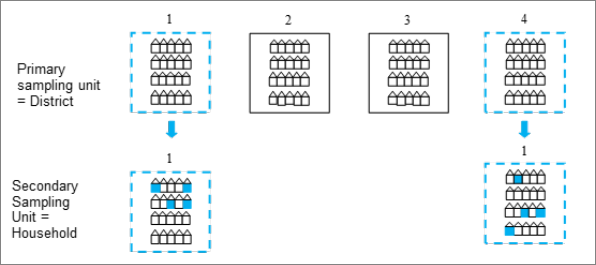
\includegraphics{pics/cluster.png}

}

\caption{Figure 1: Clustering in two stage sampling}

\end{figure}

Figure 1 provides a simplified illustration of clustering with four
districts as Primary Sampling Units (PSUs). The dotted lines indicate
that districts 1 and 4 have been selected to be in the sample. A second
stage of sampling follows where within the two sampled districts samples
of households are taken. As a result, of this design we obtain a sample
of households but these households are clustered within a sample of
districts.

Subsequently drawing of either further clusters or final sample members
take place within the already selected clusters. These higher level
clusters, ie those at which the first random draw happened as known as
Primary Sampling Units (PSUs). In large scale surveys the PSUs are often
geographical areas.

\textbf{Household level clustering}

A lesser discussed aspect of clustering arise if all individuals at a
sampled household are selected. Imagine we are estimating the proportion
of individuals who are born outside the UK from a population of 100
people who live in 50 households. We would expect people who are born
outside the UK to be more likely to live together than if they were
scattered randomly across all households. Instead we will find them
`clustered' within households, with some households being wholly
overseas born, some mixed and most wholly UK born.

e.g.~

\begin{verbatim}
Household 1: 1 UK born individuals 
Household 2: 3 UK born 
Household 3: 2 Overseas born 
Household 4: 6 UK born 
Household 5: 1 Overseas born, 1 UK born 
Household 6: 2 UK born 
Household 7: 1 UK born 
Household 8: 1 UK born 
Household 9: 5 Overseas born 
Household 10: 3 UK born 
\end{verbatim}

And so on\ldots{}

This means that if we are selecting only one in ten of the households
for our sample we might expect the sample to be less accurate in
predicting the proportion of our population who were born outside the UK
than if we had sampled individuals at random.

More generally, using clustering comes at the cost of making the
sampling coarser in the sense that we are shrinking the size of the
population from which it is going to be drawn - reducing its diversity -
which in turn makes the estimates produced from the resulting data less
precise. We will cme back to this in the next section.

\hypertarget{stratification}{%
\subsection{1.2 Stratification}\label{stratification}}

In stratified sampling, the population is divided into groups, or
strata, and a sample of units is selected from each. Stratified sampling
ensures the sample includes a certain proportion of units from the
selected groups that may have been missed otherwise. By contrast with
clustering strata are constructed so as to maximise their internal
homogeneity.

\begin{figure}

{\centering 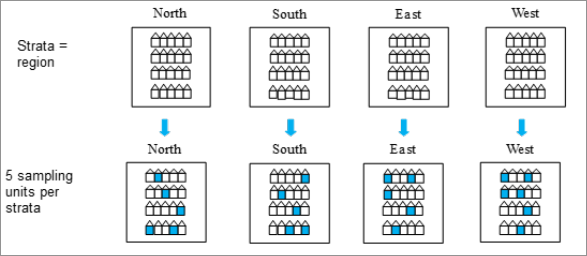
\includegraphics{pics/strata.png}

}

\caption{Figure 2: An example of stratified sampling}

\end{figure}

Figure 2 provides a simplified example where the population is divided
into four strata: North, South, East and West. Within each strata five
sampling units (represented by houses) are selected.

Common stratification characteristics used in UK surveys are
geographical (e.g.~Government Office Regions); socio-economic
(e.g.~proportion of people in the area in certain occupations; car
ownership) or demographic (e.g.~proportion of people who are pensioners,
population density). Such information is usually obtained from Census
data.

It is considered that overall stratification by improving the
representativeness of potentially less represented or harder to reach
groups increases the precision of surveys.

\#\#1.3 Proportional vs non proportional stratification In simple random
sample each element drawn from the sampling frame have an equal
selection probability, therefore the sampling fraction is \(n/N\) with
\(n\) the sample size and N the population size. This can either be
achieved by directly selecting sample units at random or by choosing a
random start and an interval.

In the context of stratified sampling \emph{proportionate
stratification} refers to case where the same sampling fraction is used
for elements within all stratum: ie \(n_h/N_h\). We can see this in
Figure 2 as the same proportion of units is selected for all strata with
a sampling fraction of \(1/4\).

It is sometimes necessary to use \emph{disproportionate stratification}
where the sampling fraction varies across strata. This method is used to
increase the numbers of a specific group in the population and is useful
when a sub-population of interest is numerically small, like less
populated areas or ethnic minority groups. In such a case,
\(n_h/N_h>n_{h+1}/N_{h+1}\): the sampling fraction in stratum \(h\) is
larger ie we are proportionally drwing more units in that stratum
relative to its size, than in stratum \(h+1\). For example the British
Election Study 2010 respondents from an ethnic minority background were
over-sampled as too little was known about ethnic minority voting
behaviour. Disproportionate stratification will mean some groups are
over-represented in the sample.

(\textbf{PierreWal?}): I think we should remove commented out content

\hypertarget{design-based-inference-from-social-surveys}{%
\section{2 Design-based inference from social
surveys}\label{design-based-inference-from-social-surveys}}

As we have just seen, collecting data about people at random is not
necessarily straightforward to achieve. There is no such thing as a
sampling frame - a list of all UK residents to pick from - and even if
there were one, some people would be less likely to take part to survey
than others. As a result most UK social surveys rely on sampling
techniques such as multi-stage clustering and stratification, alongside
sampling proportional to size in order to strike a compromise between
tackling non response, unequal probability of selection, improving the
representativeness of hard to reach groups while keeping fieldwork costs
down.

Conducting inference consist in estimating parameters - quantities of
interests from surveys, whether point estimates such as means or median
and/or measures of their degree of precision such as confidence
intervals or standard errors. Both are potentially affected by the
sample design that was implemented during data collection, and need to
be adapted accordingly. It is generally accepted that by increasing the
sampling fraction for groups, stratification improves the precision of
estimates, whereas by in effect removing part of the population from the
sample, clustering will negatively impact precision. Since most survey
use a combination of both, the impact of survey design will depend on
the quantity and the subgroups of the population estimated, if any.
Furthermore using weights to reflect non-response or unequal probability
of selection also affect the precision of estimations - often negatively
- and this should ideally be also taken into account when computing
estimates.

Traditional textbooks or introductory courses tend to leave out this
aspect, which may give a false impression of simplicity to users. There
are traditionally two main ways to produce population estimates from
surveys while accounting for sample design: either by directly using
methods that correct estimates for the characteristics of the sample -
also known a \emph{design-based estimation} - or by modelling the effect
of sample design - the \emph{model-based approach}. Both have advantages
and downsides, but for now we will only focus on the design based
approach as it tends to be more straightforward to use.

\hypertarget{survey-design-variables}{%
\subsection{2.1 Survey design variables}\label{survey-design-variables}}

\emph{Weights} are a special type of numeric variables included in
survey datasets, whose value tends to be the inverse of the relative
`importance' of sampled observations. They are designed to prevent
estimates from being biased, that is reflecting a value that is not
representative of the population. They are usually made of at least two
components:

\begin{itemize}
\item
  a \emph{design} component that accounts for issues of unequal
  probability of selection of sample members resulting from survey
  design;
\item
  a \emph{non-response} component, correcting for (known) lower
  propensity to take part to surveys among certain categories of
  respondents.
\end{itemize}

Rather confusingly, these components are sometimes labelled `weights' in
their own right, even if in practice they are most of the time merged
into a single variable.

Survey weights may also be rescaled in order to inflate sample counts to
population totals thus becoming \emph{grossing weights} which enable
estimating populations size. In that sense the numerical values of the
weights attached to observations are an indication of the number of
units these observation `represent' in the population.

Computation of weights rely on calibration algorithms that optimise the
conditional distribution of the weighting variables given the sample
size (for example the conditional distribution of people by age, gender
and economic status) with a view to strike a balance between minimising
standard errors and maximising representativeness.

\emph{Survey design variables} typically consist of identifiers for the
strata and/or clusters used when the sample was drawn, especially the
Primary Sampling Units (PSU) used during the sampling process. Used in
conjunction with weights, they enable researchers to produce more
accurate estimates.

\hypertarget{design-effects-and-design-factors}{%
\subsection{2.2 Design effects and design
factors}\label{design-effects-and-design-factors}}

Whereas most surveys curated by UKDS include weights, survey design
variables are not always provided by data producers often due to data
protection concerns. This leaves users with having to rely on
alternative solutions to reduce variance estimation bias. \emph{Design
effect} (also know as DEFF or \(D_{eff}\)) and/or Design factors
(\(D_{eft}\)) may provide a partial solution in such scenarios.
\(D_{eff}\) and \(D_{eft}\) are two versions of a coefficient which
attempts to measure the extent to which the standard error of an
estimate given the current survey design differs from what it would have
been under simple random sampling (Kish 1995). They can therefore be
used to broadly assess how sample design affect the precision of a
particular set of estimates as well as enabling users to manually
correct standard errors and confidence intervals produced under the
assumption of simple random sampling. Formally, the \(D_{eff}\) is
defined as the ratio of the variance of an estimated parameter of
interest to the same variance computed under the assumption of simple
random sampling.The \(D_{eft}\) by contrast is the square root of the
Design Effect. A \(D_{eff}\) with a value \(<1\) indicates an smaller
variance than under SRS, therefore an improvement in precision, whereas
a value \(>1\) indicates a loss of precision. Data producers sometimes
provides Design factor estimates that can be used to correct biased
standard error or confidence intervals.

\hypertarget{the-practice-of-inference-things-to-keep-in-mind}{%
\section{3. The practice of inference: things to keep in
mind}\label{the-practice-of-inference-things-to-keep-in-mind}}

The variability (and therefore the degree of precision with which they
can be estimated) of point estimates is contingent on survey weights and
survey design. Although therefore the optimum approach to estimating
population parameters from surveys relies on using both weights and
survey design variables, it is not always possible to go down that path.
In practice, trade-offs have to be made depending on several factors.
Let us briefly consider them.

\hypertarget{data-availability}{%
\subsection{3.1 Data availability}\label{data-availability}}

Most UKDS datasets are available under \emph{End User License (EUL)}.
This presents the advantage of enabling large numbers of users to access
data with a minimal level of formalities to go through but comes at the
significant cost that survey design variables are often not included by
the data producer, due to concerns about the risk of personal
information disclosure. There are notable exceptions, such as for
example the British Social Attitudes survey which does include survey
design variables in some of its releases.

For a number of key studies such as the Labour Force Survey or the
Family Resources Survey, users may apply for access to a version of the
data that includes survey design information via the (virtual) SecureLab
or at the UKDS Safe Room. Application for access to these facilities can
be a lengthy process, and not practically feasible for all researchers,
in particular those outside academia or large organisations. More
information is available on the
\href{https://ukdataservice.ac.uk/help/access-policy/types-of-data-access/}{UKDS
website}. There are also a large number of studies for which such
controlled access is not available. The consequence is that in a
significant number of cases, there will inevitably be limitations to the
level of precision of the estimates most will be able to produce.

\hypertarget{sensitivity-of-the-analysis}{%
\subsection{3.2 Sensitivity of the
analysis}\label{sensitivity-of-the-analysis}}

Not all analyses necessarily require the highest degree of precision.
Reflecting on the stakes of their intended analysis will help users
decide how important it is to strive to use the most robust estimation
technique available or instead to settle for one that is `good enough'.
Typical usages of survey data could be seen as lying on a continuum
ranging from `playing with the data' to producing numbers that will be
subject to public scrutiny, or that will be used in policymaking. The
latter require such a degree of precision -- for example when publishing
official population estimates or writing a research article, other less
so -- for instance when exploring data or preparing examples for
teaching. In the former cases, users may simply need to get a rough idea
of a population estimate or the interval within which it may lie.

\hypertarget{complexity-of-the-analysis}{%
\subsection{3.3 Complexity of the
analysis}\label{complexity-of-the-analysis}}

What an analysis actually entails will help determine whether accessing
survey design variables is crucial or not. Estimation involving small
numbers of observations will be more at risk of providing incorrect
estimates if survey design variables are not taken into account.
Similarly, interest for specific subgroups of the population (also known
as domains) rather than the population as a whole will involve more
complex estimation techniques as domain estimation needs to account for
the distribution of weights in the whole population, not just for the
subgroup of interest.

These analytical scenarios could be seen as lying on a continuum ranging
from producing simple univariate descriptive estimates for the
population as a whole to complex estimation of small groups
characteristics and/or multivariate analysis. The former is conceptually
and practically more straightforward than the latter. In some cases the
estimates of interest may already have been published by the data
producer using the adequate estimation techniques and the full
information available. Data producers may also have published
\emph{design factors} ie numbers allowing to adjust the precision of
estimates produced without survey design variables. Examples of such
design factors for the Labour Force Survey and the Family Resources
Surveys are provided below.

\hypertarget{software-issues}{%
\subsection{3.4 Software issues}\label{software-issues}}

Most statistical analysis software include commands specifically
designed to analyse survey data: such is the case of the R \emph{Survey}
package, the SPSS \emph{Complex Survey} add-on and Stata's \emph{svy:}
set of commands. However, because weighting can be used in other
contexts than inference from surveys, most statistical software also
have options for directly weighting estimation commands ``on the fly''
outside of procedures accounting for survey design. This can lead some
users to solely rely on weighted commands without explicitly declaring
the survey design in their analysis which potentially raises issues:

\begin{itemize}
\item
  Whereas weighted commands will most of the time compute the correct
  point estimates, they will also silently produce biased estimates of
  their precision (standard errors or confidence intervals), based on
  the incorrect assumption that the sample was collect via simple random
  sampling. Depending on the survey design, this will lead to under- or
  over- estimation of standard errors and confidence intervals, and
  could affect the validity of statistical tests, in particular if small
  groups within the population are involved.
\item
  In addition, there are specific cases where estimation of standard
  errors and confidence intervals will be not just biased but wholly
  incorrect: the standard (ie command-based) weighting procedure of SPSS
  ans SAS relies on population rather than sample totals to compute
  them, which results in unrealistic values.
\item
  Software such as Stata does not allow users to directly compute
  confidence interval or use sampling weights outside of survey
  commands. This may lead users to rely on `quick and dirty' tricks that
  will help them quickly produce weighted point estimates, with
  incorrect standard errors.
\end{itemize}

\hypertarget{what-are-we-in-fact-estimating}{%
\subsection{3.5 What are we in fact
estimating?}\label{what-are-we-in-fact-estimating}}

Users can prioritise producing weighted point estimates over estimating
their precision and the factors that influence it - chiefly survey
design variables. It can be tempting indeed to consider that the goal of
statistical inference mainly consists in producing `representative'
point estimates of a quantity of interest such as the `mean weight of
adult males', the `median poverty rate', or the value of some regression
coefficient in a multivariate study with estimates of their precision a
secondary consideration, or a qualifier of the point estimate.

This is potentially risky. Point estimates can be at the same time
representative \emph{and} imprecise, and therefore carry little
practical meaning. It could also be argued that focusing too narrowly on
single value population estimates implicitly entertains the idea that
such unique, `true' value exist. As these in fact constantly vary,
different surveys will return inevitably different estimates.

Instead, conceiving from the start these two aspects as a single reality
-- a range of plausible values we think a parameter of interest can take
in the population, with a certain degree of confidence -- could help
alleviate such a risk and most importantly provide a more accurate
reflection of the reality we seek to describe. Striving to produce
confidence intervals whenever it makes sense to do so will help the
notion that precision and therefore inevitably survey design are key to
robust estimation.

\hypertarget{statistical-inference-from-survey-data-in-practice}{%
\section{4. Statistical inference from survey data in
practice}\label{statistical-inference-from-survey-data-in-practice}}

\emph{Ultimately there should be a flowchart here or in the next
section}

This section provides practical recommendations for robust inference
taking into account the factors highlighted in Section 3. In general,
four strategies are available when conducting population inference from
survey data. They are listed below by order of recommendation by the UK
Data Service:

\begin{enumerate}
\def\labelenumi{\arabic{enumi}.}
\tightlist
\item
  Estimation accounting for weights and survey design using
  survey-specific commands
\item
  Estimation accounting for weights only using survey-specific commands
\item
  Estimation using weighted standard commands
\item
  (Unweighted estimation)
\end{enumerate}

\begin{itemize}
\item
  \emph{Strategy 1}, using weights alongside survey design variables
  when conducting statistical inference is the statistically most robust
  way to compute population estimates with survey data and should be
  prioritised by users whenever possible. In real life research however,
  this option is not always available. Accessing survey design variables
  can prove challenging as they are not always provided by data
  producers or may require applying for a special version of the data,
  which may prove time consuming.
\item
  In the absence of survey design information, \emph{Strategy 2} should
  be considered the second best option. The value of point estimates are
  likely to be identical to those produced under Strategy 1, but the
  confidence intervals/standard errors will be biased -- ie too narrow
  or wide depending on the survey design, which should be explicitly
  mentioned alongside the results. Information from the data
  documentation should provide information about how results may be
  affected. Using survey-specific estimation commands even in the
  absence of survey design variables is a recommended option over simply
  applying weights to standard commands, as it will avoid getting
  incorrect estimates (SAS and SPSS), is the only option available for
  computation with survey weights or obtaining confidence intervals
  (Stata), or coherent survey data analysis (R). In addition, it might
  be possible to correct `by hand' biased standard errors or confidence
  interval using data producer-provided design factors.
\item
  It can be understandable that when survey design variables are not
  available some users privilege \emph{Strategy 3} which tend to focus
  on producing weighted estimates using standard commands and give
  little consideration to the methodological implication of this
  approach. Whereas point estimates are likely to be identical to those
  produced under Strategy 1 and 2, SAS and SPSS users are likely to
  produce incorrect confidence intervals/standard errors. R and Stata
  users might get standard errors and confidence intervals that are
  close to those produced using Strategy 2, but there is not guarantee
  that this will be the case. Overall UKDS only recommend following this
  strategy in case of low sensitivity analysis.
\item
  As population estimates produced without weights or survey design
  variables will almost certainly be unreliable \emph{Strategy 4} should
  be discouraged except when data usage is purely descriptive. For
  example when teaching non-inferential (ie descriptive) statistical
  techniques.
\end{itemize}

\hypertarget{medium-to-high-sensitivity-analysis-workflow}{%
\subsection{4.1 Medium to high sensitivity analysis:
workflow}\label{medium-to-high-sensitivity-analysis-workflow}}

Most of the time survey researchers or data analysts are required to
produce a confidence interval or provide an indication of the degree of
precision of their point estimate, usually with standard errors, whose
correct estimation depends on the amount of information held about the
survey design.

\begin{enumerate}
\def\labelenumi{\arabic{enumi}.}
\tightlist
\item
  \textbf{If survey design variables are available} a typical workflow
  could involve (see examples in Section 5):
\end{enumerate}

\begin{itemize}
\tightlist
\item
  Finding out about the survey design and identify the relevant weights
  and survey design variables in the data documentation;
\item
  Declaring the survey design using software-specific commands
\item
  Producing the estimates of interest, using survey design specific
  estimation commands available
\item
  Documenting the confidence interval for the estimate of interest or
  alternatively the point estimates \emph{and} its standard error.
\item
  If required, provide a brief discussion of the possible source of bias
  of the results (specifically under/over estimation of the uncertainty
  of the estimates)
\end{itemize}

\begin{enumerate}
\def\labelenumi{\arabic{enumi}.}
\setcounter{enumi}{1}
\item
  If the survey design variables are not included in the EUL version of
  the data but are available under controlled access: perform a cost vs
  benefits analysis of applying for controlled access for instance via
  the UKDS SecureLab, a process that can take some time. Information
  about how to apply for Secure Lab Access is available
  \href{https://ukdataservice.ac.uk/find-data/access-conditions/secure-application-requirements/apply-to-access-ons-data}{on
  the UKDS website}.
\item
  If the \textbf{survey design variables such as strata, cluster, or
  primary sampling unit are not available} an alternative workflow could
  consist in:
\end{enumerate}

\begin{itemize}
\item
  If the user is interested in overall population characteristics,
  checking whether the estimates of interest may already have been
  published by the data producer, in which case they may be directly
  cited instead of computed from data.
\item
  Finding out about the survey design in the data documentation and
  identify the weights variable ;
\item
  Declaring the survey design as simple random sampling using
  software-specific commands
\item
  Producing the estimates of interest, using survey design specific
  estimation commands available
\item
  Checking whether the data producer has published design factors that
  could be used to remedy to biased confidence intervals/ standards
  errors computed without survey design variables (for example design
  factors computed for the same population at another point in time). A
  design factor is a number by which to multiply standard errors
  estimated under the assumption of simple random sampling, that will
  adjust it for survey design characteristics.
\item
  Documenting the resulting confidence interval for the estimate of
  interest or alternatively the point estimates \emph{and} its standard
  error.
\item
  If no design factors are available for the estimates of interest, an
  explicit mention of the likely nature and cause of bias is good
  practice ie under estimation in case of cluster sampling, over
  estimation in case of stratified sample, usually available from the
  survey documentation. The wider the initial confidence interval (ie
  computed under SRS assumptions) the larger the likely bias. Or from
  another perspective, the smaller the (sub)sample, the larger the
  likely bias. In cases of conducting significance testing with small
  subsample or groups, it would be a good practice to only consider test
  outcomes significant at P\textless.01 or p\textless.001.
\end{itemize}

\begin{enumerate}
\def\labelenumi{\arabic{enumi}.}
\setcounter{enumi}{3}
\tightlist
\item
  Computing SDI estimates for subpopulations (also known as `domains')
  rather than for the population as a whole requires extra precautions.
  This is the case for example when we are interested in the mean age by
  employment status, or some other categories, or alternatively, in
  analyses restricted to a subset of the population (for example only
  those in employment). The key differences is that when computing
  domain estimates we are in fact producing estimates about a group of
  the population whose size we also need to estimate. This requires
  ensuring that the whole distribution of weights in the sample is taken
  into account, not just the weights values for the groups we are
  interested in. Failure to do so might result in computing incorrect
  point estimates and standard errors/confidence intervals. SDI commands
  in statistical software are designed to tackle this potential issue.
\end{enumerate}

\hypertarget{lower-sensitivity-analysis}{%
\subsection{4.2 Lower sensitivity
analysis}\label{lower-sensitivity-analysis}}

The UKDS does not recommend using command-specific or casual weighting
for inferential analysis, but there are circumstances where this will be
the only option available to users. There are also cases when users are
not interested in knowing about the uncertainty of their estimates (ie
their confidence interval, standard errors of point estimates, or
conduct statistical testing), for example because they are simply
learning or teaching basic statistical concepts or how to use software.

In such cases, it can be acceptable to compute point estimates by
applying weights to commands that accepts them, without using survey
design specific functions. Most of these will provide the correct point
estimate. By default however, some statistical software will also
provide an estimate of standard errors or confidence intervals, which is
likely to be misleading as they `silently' assume simple random
sampling, and in some cases will carry out computation with population
(ie grossed) totals, resulting in the incorrect values.

(\textbf{PierreWal?}) : here too

\hypertarget{r-examples}{%
\section{5. R examples}\label{r-examples}}

The R \emph{Survey} package (Lumley 2023) provides a comprehensive set
of functions for computing point and variance estimates from survey
data. At the same time, R Base does not provide a unified sets of
commands or syntax for computing weighted estimates. Implementation of
statistical theory may vary between packages, but algorithms are usually
described in detail in the package documentation.

In this example, we will practice statistical inference with data from
the
\href{https://beta.ukdataservice.ac.uk/datacatalogue/studies/study?id=8450}{2017
British Social Attitudes Survey (BSA)} taking into account weights and
survey design variables. Please note that at the time of writing this
document only some issues of the BSA include survey design variables.

\hypertarget{identifying-the-survey-design-and-variables}{%
\subsection{5.1 Identifying the survey design and
variables}\label{identifying-the-survey-design-and-variables}}

We first need to find out about the survey design that was used in the
2017 BSA, and the design variables that are made available in the
dataset. Such information can usually be found in the documentation that
comes together with the data under the \texttt{mrdoc/pdf} folder.

\textbf{Question 1} What is the design that was used in this survey (ie
how many stages were there, and what were the units sampled). What were
the primary sampling units; the strata (if relevant)?

Now that we are a bit more familiar with the way the survey was
designed, we need to try and identify the design variables we can
include when producing estimates. The information can usually be found
in the user manual or the data dictionary available under
\texttt{mrdoc/ukda\_data\_dictionaries.zip} The file may need to be
decompressed separately.

\textbf{Question 2} What survey design variables are available? Are
there any ones that are missing -- if so which ones? What is the name of
the weights variables?

\hypertarget{specifying-the-survey-design}{%
\subsection{5.2 Specifying the survey
design}\label{specifying-the-survey-design}}

\begin{Shaded}
\begin{Highlighting}[]
\FunctionTok{rm}\NormalTok{(}\AttributeTok{list=}\FunctionTok{ls}\NormalTok{())}
\FunctionTok{library}\NormalTok{(dplyr) }\DocumentationTok{\#\#\# Data manipulation functions}
\FunctionTok{library}\NormalTok{(haven) }\DocumentationTok{\#\#\# Importing stata/SPSS files}
\FunctionTok{library}\NormalTok{(Hmisc) }\DocumentationTok{\#\#\# Extra statistical functions}
\FunctionTok{library}\NormalTok{(survey) }\DocumentationTok{\#\#\# Survey design functions}
\FunctionTok{library}\NormalTok{(kableExtra) }\DocumentationTok{\#\#\# Survey design functions}

\NormalTok{bsa17}\OtherTok{\textless{}{-}}\FunctionTok{read\_spss}\NormalTok{(}\StringTok{"\textasciitilde{}/Dropbox/work/UKDS/data/UKDA{-}8450{-}spss/spss/spss25/bsa2017\_for\_ukda.sav"}\NormalTok{)}
\FunctionTok{dim}\NormalTok{(bsa17)}
\end{Highlighting}
\end{Shaded}

\begin{verbatim}
[1] 3988  580
\end{verbatim}

We can specify the survey design earlier identified in the data
documentation: using \texttt{Spoint} as Primary Sampling Unit,
\texttt{StratID} as strata, and \texttt{WtFactor} as weights. R does
this by creating a \texttt{svydesign} object, ie a survey design
informed version of the data, which will be used for subsequent
estimation.

\begin{Shaded}
\begin{Highlighting}[]
\NormalTok{bsa17.s}\OtherTok{\textless{}{-}}\FunctionTok{svydesign}\NormalTok{(}\AttributeTok{ids=}\SpecialCharTok{\textasciitilde{}}\NormalTok{Spoint, }\AttributeTok{strata=}\SpecialCharTok{\textasciitilde{}}\NormalTok{StratID, }\AttributeTok{weights=}\SpecialCharTok{\textasciitilde{}}\NormalTok{WtFactor,}\AttributeTok{data=}\NormalTok{bsa17)}
\FunctionTok{class}\NormalTok{(bsa17.s)}
\end{Highlighting}
\end{Shaded}

\begin{verbatim}
[1] "survey.design2" "survey.design" 
\end{verbatim}

\hypertarget{mean-age-and-its-95-confidence-interval}{%
\subsection{5.3 Mean age and its 95\% confidence
interval}\label{mean-age-and-its-95-confidence-interval}}

We can now produce a first set of estimates using this information and
compare them with those we would have got without accounting for the
survey design. We will compute the average (ie mean) age of respondents
in the sample. We will need to use \texttt{svymean()}

\begin{Shaded}
\begin{Highlighting}[]
\FunctionTok{svymean}\NormalTok{(}\SpecialCharTok{\textasciitilde{}}\NormalTok{RAgeE,bsa17.s)}
\end{Highlighting}
\end{Shaded}

\begin{verbatim}
        mean     SE
RAgeE 48.313 0.4236
\end{verbatim}

By default \texttt{svymean()} computes the standard error of the mean.
We need to\\
embed it within \texttt{confint()} in order to get a confidence
interval.

\begin{Shaded}
\begin{Highlighting}[]
\FunctionTok{confint}\NormalTok{(}\FunctionTok{svymean}\NormalTok{(}\SpecialCharTok{\textasciitilde{}}\NormalTok{RAgeE,bsa17.s)) }\DocumentationTok{\#\#\# Just the confidence interval...}
\end{Highlighting}
\end{Shaded}

\begin{verbatim}
         2.5 %  97.5 %
RAgeE 47.48289 49.1433
\end{verbatim}

\begin{Shaded}
\begin{Highlighting}[]
\FunctionTok{round}\NormalTok{(}
  \FunctionTok{c}\NormalTok{(}
    \FunctionTok{svymean}\NormalTok{(}\SpecialCharTok{\textasciitilde{}}\NormalTok{RAgeE,bsa17.s),}
    \FunctionTok{confint}\NormalTok{(}\FunctionTok{svymean}\NormalTok{(}\SpecialCharTok{\textasciitilde{}}\NormalTok{RAgeE,bsa17.s))}
\NormalTok{    ),}
  \DecValTok{1}\NormalTok{)}\DocumentationTok{\#\#\# Estimate and CI, rounded}
\end{Highlighting}
\end{Shaded}

\begin{verbatim}
RAgeE             
 48.3  47.5  49.1 
\end{verbatim}

\textbf{Question 3} What would be the consequences of weighing but not
accounting for the sample design; not using weights and accounting for
the sample design when:

\begin{itemize}
\tightlist
\item
  inferring the mean value of the population age?
\item
  inferring the uncertainty of our estimate of the population age?
\end{itemize}

\hypertarget{computing-a-proportion-and-its-95-confidence-interval}{%
\subsection{5.4 Computing a proportion and its 95\% confidence
interval}\label{computing-a-proportion-and-its-95-confidence-interval}}

We can now similarly compute the distribution of a categorical variable
in the population by estimating proportions (or percentages), for
instance, the proportion of people who declare that they are interested
in politics. This is the \texttt{Politics} variable in the BSA. It has
five categories ranging from 1 `A great deal' to 5- `Not at all'. We
could recode 1 and 2 - \texttt{quite\ a\ lot} into `Significantly', but
since we are only interested in estimating the confidence intervals, we
will select the relevant values `on the go'.

\begin{Shaded}
\begin{Highlighting}[]
\FunctionTok{attr}\NormalTok{(bsa17}\SpecialCharTok{$}\NormalTok{Politics,}\StringTok{"label"}\NormalTok{)     }\DocumentationTok{\#\#\# Phrasing of the question}
\end{Highlighting}
\end{Shaded}

\begin{verbatim}
[1] "How much interest do you have in politics?"
\end{verbatim}

\begin{Shaded}
\begin{Highlighting}[]
\FunctionTok{attr}\NormalTok{(bsa17}\SpecialCharTok{$}\NormalTok{Politics,}\StringTok{"labels"}\NormalTok{)     }\DocumentationTok{\#\#\# Value labels}
\end{Highlighting}
\end{Shaded}

\begin{verbatim}
skip, version off route     Item not applicable       ... a great deal, 
                     -2                      -1                       1 
           quite a lot,                   some,          not very much, 
                      2                       3                       4 
       or, none at all?              Don`t know                 Refusal 
                      5                       8                       9 
\end{verbatim}

\begin{Shaded}
\begin{Highlighting}[]
\FunctionTok{table}\NormalTok{(}\FunctionTok{as\_factor}\NormalTok{(bsa17}\SpecialCharTok{$}\NormalTok{Politics)) }\DocumentationTok{\#\#\# Sample distribution}
\end{Highlighting}
\end{Shaded}

\begin{verbatim}

skip, version off route     Item not applicable       ... a great deal, 
                      0                       0                     739 
           quite a lot,                   some,          not very much, 
                    982                    1179                     708 
       or, none at all?              Don`t know                 Refusal 
                    379                       1                       0 
\end{verbatim}

\textbf{Note}: Changes in a data frame are not automatically transferred
into \texttt{svydesign} objects used for inferences. We therefore need
to recreate it each time we create or recode a variable.

\begin{Shaded}
\begin{Highlighting}[]
\FunctionTok{round}\NormalTok{(}\DecValTok{100}\SpecialCharTok{*}\FunctionTok{prop.table}\NormalTok{(}\FunctionTok{svytable}\NormalTok{(}\SpecialCharTok{\textasciitilde{}}\NormalTok{(Politics}\SpecialCharTok{==}\DecValTok{1} \SpecialCharTok{|}\NormalTok{ Politics}\SpecialCharTok{==}\DecValTok{2}\NormalTok{),bsa17.s)),}\DecValTok{1}\NormalTok{)}
\end{Highlighting}
\end{Shaded}

\begin{verbatim}
Politics == 1 | Politics == 2
FALSE  TRUE 
   57    43 
\end{verbatim}

Let us now compute the confidence intervals for these proportions.
Traditional statistical software compute these without giving us an idea
of the underlying computations going on. Doing this in R requires more
coding, but also a better understanding of what is actually estimated.

Confidence intervals for proportions of categorical variables are
usually computed as a sequence of binomial/dichotomic estimations -- ie
one for each category. In R this needs to be specified explicitly via
the \texttt{svyciprop()} and \texttt{I()} functions. The former actually
computes the proportion and its confidence interval (by default 95\%),
whereas the latter allows us to define the category we are focusing on.

\begin{Shaded}
\begin{Highlighting}[]
\FunctionTok{svyciprop}\NormalTok{(}\SpecialCharTok{\textasciitilde{}}\FunctionTok{I}\NormalTok{(Politics}\SpecialCharTok{==}\DecValTok{1} \SpecialCharTok{|}\NormalTok{ Politics}\SpecialCharTok{==}\DecValTok{2}\NormalTok{),bsa17.s)}
\end{Highlighting}
\end{Shaded}

\begin{verbatim}
                                        2.5% 97.5%
I(Politics == 1 | Politics == 2) 0.430 0.411  0.45
\end{verbatim}

\begin{Shaded}
\begin{Highlighting}[]
\FunctionTok{round}\NormalTok{(}\DecValTok{100}\SpecialCharTok{*}
        \FunctionTok{c}\NormalTok{(}\FunctionTok{prop.table}\NormalTok{(}\FunctionTok{svytable}\NormalTok{(}\SpecialCharTok{\textasciitilde{}}\NormalTok{(Politics}\SpecialCharTok{==}\DecValTok{1} \SpecialCharTok{|}\NormalTok{ Politics}\SpecialCharTok{==}\DecValTok{2}\NormalTok{),bsa17.s))[}\DecValTok{2}\NormalTok{],}
\FunctionTok{attr}\NormalTok{(}\FunctionTok{svyciprop}\NormalTok{(}\SpecialCharTok{\textasciitilde{}}\FunctionTok{I}\NormalTok{(Politics}\SpecialCharTok{==}\DecValTok{1} \SpecialCharTok{|}\NormalTok{ Politics}\SpecialCharTok{==}\DecValTok{2}\NormalTok{),bsa17.s),}\StringTok{"ci"}\NormalTok{)),}\DecValTok{1}
\NormalTok{)}
\end{Highlighting}
\end{Shaded}

\begin{verbatim}
 TRUE  2.5% 97.5% 
 43.0  41.1  44.9 
\end{verbatim}

\textbf{Question 4} What is the proportion of respondents aged 17-34 in
the sample, as well as its 95\% confidence interval? You can use
\texttt{RAgecat5}

\hypertarget{computing-domain-estimates}{%
\subsection{5.5 Computing domain
estimates}\label{computing-domain-estimates}}

Computing domain estimates, that is estimates for subgroups adds a layer
of complexity to the above example. They key point is that as weights
were designed using the whole of the sample, computing estimates, in
particular confidence intervals or standard errors for part of the
sample, therefore using a fraction of these weights may affect the
estimates. Instad it is recommended to use commands that take into
account the entire distribution of the weights.

In R, the command that does this is \texttt{svyby()}

For instance, if we would like to compute the mean age of BSA
respondents by Government Office Regions, we need to specify:

\begin{itemize}
\tightlist
\item
  The outcome variable whose estimate we want to compute: ie
  \texttt{RAgeE}
\item
  The grouping variable(s) \texttt{GOR\_ID}
\item
  The estimate function we are going to use here: \texttt{svymean}, the
  same as we used before
\item
  And the type of type of variance estimation we would like to see
  displayed ie standard errors or confidence interval
\end{itemize}

\begin{Shaded}
\begin{Highlighting}[]
\FunctionTok{round}\NormalTok{(}
      \FunctionTok{svyby}\NormalTok{(}\SpecialCharTok{\textasciitilde{}}\NormalTok{RAgeE,}\AttributeTok{by=}\SpecialCharTok{\textasciitilde{}}\FunctionTok{as\_factor}\NormalTok{(GOR\_ID),svymean,}\AttributeTok{design=}\NormalTok{bsa17.s,}\AttributeTok{vartype =} \StringTok{"ci"}\NormalTok{)[}\SpecialCharTok{{-}}\DecValTok{1}\NormalTok{]}
\NormalTok{      ,}\DecValTok{1}\NormalTok{)}
\end{Highlighting}
\end{Shaded}

\begin{verbatim}
                           RAgeE ci_l ci_u
A North East                46.1 43.6 48.6
B North West                49.6 47.3 52.0
D Yorkshire and The Humber  48.0 45.2 50.8
E East Midlands             48.6 45.9 51.3
F West Midlands             48.1 45.0 51.2
G East of England           49.0 46.0 52.0
H London                    45.0 43.0 46.9
J South East                48.0 45.1 50.8
K South West                53.4 51.5 55.2
L Wales                     49.1 45.1 53.1
M Scotland                  47.3 44.7 50.0
\end{verbatim}

\emph{Note:} we used \texttt{{[}-1{]}} from the object created by
\texttt{svyby()} in order to remove a column with alphanumeric values
(the region names), so that we could round the results without getting
an error.

Our inference seem to suggest that the population in London is among the
youngest in the country, and that those in the South West are among the
oldest -- their respective 95\% confidence intervals do not overlap. We
should not feel so confident about differences between London and the
South East for example, as the CIs partially overlap.

We can follow a similar approach with proportions: we just need to
specify the category of the variable we are interested in as an outcome,
for instance respondents who are significantly interested in politics,
and replace \texttt{svymean} by \texttt{svyciprop}.

\begin{Shaded}
\begin{Highlighting}[]
\FunctionTok{round}\NormalTok{(}
      \DecValTok{100}\SpecialCharTok{*}
      \FunctionTok{svyby}\NormalTok{(}\SpecialCharTok{\textasciitilde{}}\FunctionTok{I}\NormalTok{(Politics}\SpecialCharTok{==}\DecValTok{1} \SpecialCharTok{|}\NormalTok{ Politics}\SpecialCharTok{==}\DecValTok{2}\NormalTok{),}
            \AttributeTok{by=}\SpecialCharTok{\textasciitilde{}}\FunctionTok{as\_factor}\NormalTok{(GOR\_ID),}
\NormalTok{            svyciprop,}
            \AttributeTok{design=}\NormalTok{bsa17.s,}
            \AttributeTok{vartype =} \StringTok{"ci"}\NormalTok{)[}\SpecialCharTok{{-}}\DecValTok{1}\NormalTok{],}
            \DecValTok{1}\NormalTok{)}
\end{Highlighting}
\end{Shaded}

\begin{verbatim}
                           I(Politics == 1 | Politics == 2) ci_l ci_u
A North East                                           33.4 26.6 40.9
B North West                                           41.9 36.1 48.0
D Yorkshire and The Humber                             35.6 29.1 42.6
E East Midlands                                        36.9 32.9 41.1
F West Midlands                                        36.3 31.5 41.5
G East of England                                      47.2 41.4 53.1
H London                                               54.2 47.2 61.1
J South East                                           44.6 38.7 50.8
K South West                                           46.5 39.4 53.8
L Wales                                                38.6 27.7 50.7
M Scotland                                             42.7 36.0 49.8
\end{verbatim}

\textbf{Question 5} What is the 95\% confidence interval for the
proportion of people interested in politics in the South West? Is the
proportion likely to be different in London? In what way? What is the
region of the UK for which the precision of the estimates is likely to
be the smallest?

\textbf{Question 6} Using interest in politics as before, and three
category age \texttt{RAgecat5}:

\begin{itemize}
\item
  Produce a table of results showing the proportion of respondents
  significantly interested in Politics by age group and gender
\item
  Assess whether the age difference in interest for politics is similar
  for each gender?
\item
  Based on the data, is it fair to say that men aged under 35 tend to be
  more likely to declare themselves interested in politics than women
  aged 55 and above?
\end{itemize}

\hypertarget{inference-without-survey-design-variables-using-r}{%
\subsection{5.6 Inference without survey design variables using
R}\label{inference-without-survey-design-variables-using-r}}

\emph{Example: count and proportion of the regional population of the UK
using the LFS with End User License (EUL)}

As a rule, EUL versions of the LFS do not include sample design
variables. On the other hand they come with two weight variables:

\begin{itemize}
\tightlist
\item
  \texttt{pwt22} for estimation with the whole sample
\item
  \texttt{piwt22} for estimation using respondents currently in
  employment (typically used for earnings estimation)
\end{itemize}

Estimation without accounting for sample design will likely be biased
and should be reported as such including warnings, even if the nature
(over or underestimation of the precision) and and size are not known.
An alternative is to look for design effects tables published by the
data producer which could be used to correct for the bias.

The Office for National Statistics regularly publishes such tables for
the LFS, albeit mostly for their headline statistics. Obtaining further
design effects for subpopulations might not be straighforward. The
overall methodology is described
\href{https://www.ons.gov.uk/methodology/methodologicalpublications/generalmethodology/onsworkingpaperseries/onsmethodologyworkingpaperseriesno9guidetocalculatingstandarderrorsforonssocialsurveys\#annex-a-labour-force-survey-standard-errors-january-to-march-2015-united-kingdom}{in
this note}, and updated tables are provided
\href{Volume\%201:\%20Background\%20and\%20methodology\%20(PDF,\%201.2MB)}{on
this page}.

Let's see how this can be achieved. But first, let's produce uncorrected
`naive' estimates of the regional population.

\begin{Shaded}
\begin{Highlighting}[]
\NormalTok{lfs}\OtherTok{\textless{}{-}}\FunctionTok{read\_dta}\NormalTok{(}\StringTok{"\textasciitilde{}/Dropbox/work/UKDS/data/UKDA{-}8999{-}stata/lfsp\_aj22\_eul\_pwt22.dta"}\NormalTok{)}\SpecialCharTok{\%\textgreater{}\%}\FunctionTok{select}\NormalTok{(PWT22,PIWT22,URESMC,ILODEFR)}
\FunctionTok{names}\NormalTok{(lfs)}\OtherTok{\textless{}{-}}\FunctionTok{tolower}\NormalTok{(}\FunctionTok{names}\NormalTok{(lfs))}
\NormalTok{lfs}\SpecialCharTok{$}\NormalTok{uresmc.f}\OtherTok{\textless{}{-}}\FunctionTok{droplevels}\NormalTok{(}\FunctionTok{as\_factor}\NormalTok{(lfs}\SpecialCharTok{$}\NormalTok{uresmc))}
\NormalTok{lfs.s}\OtherTok{\textless{}{-}}\FunctionTok{svydesign}\NormalTok{(}\AttributeTok{ids=}\SpecialCharTok{\textasciitilde{}}\DecValTok{1}\NormalTok{,}\AttributeTok{weights=}\SpecialCharTok{\textasciitilde{}}\NormalTok{piwt22,}\AttributeTok{data=}\NormalTok{lfs}\SpecialCharTok{\%\textgreater{}\%}\FunctionTok{filter}\NormalTok{(ilodefr}\SpecialCharTok{==}\DecValTok{1}\NormalTok{)) }
\FunctionTok{round}\NormalTok{(}\FunctionTok{confint}\NormalTok{(}\FunctionTok{svytotal}\NormalTok{(}\SpecialCharTok{\textasciitilde{}}\NormalTok{uresmc.f,lfs.s)))}
\end{Highlighting}
\end{Shaded}

\begin{verbatim}
                                     2.5 %  97.5 %
uresmc.fTyne & Wear                 375843  544677
uresmc.fRest of Northern region     679067  875001
uresmc.fSouth Yorkshire             361987  542893
uresmc.fWest Yorkshire              892298 1139996
uresmc.fRest of Yorks & Humberside  688398  901578
uresmc.fEast Midlands              1884931 2240257
uresmc.fEast Anglia                1018147 1293525
uresmc.fInner London               1403277 1950147
uresmc.fOuter London               2061142 2573440
uresmc.fRest of South East         5133587 5816347
uresmc.fSouth West                 2150551 2532611
uresmc.fWest Midlands (met county)  921916 1255744
uresmc.fRest of West Midlands      1249939 1571219
uresmc.fGreater Manchester         1041396 1341426
uresmc.fMerseyside                  473854  749424
uresmc.fRest of North West          929920 1205848
uresmc.fWales                      1101246 1410746
uresmc.fStrathclyde                 722247 1020673
uresmc.fRest of Scotland           1356361 1750183
uresmc.fNorthern Ireland            689076  803340
\end{verbatim}

In the above example, we are working with the most commonly used flavour
of the Labour Force Survey: the quarterly edition. The specific dataset
used above is the April-July 2022 issue. Looking at the latest version
of the documentation mentioned above - Volume 1, Annex C, we can see a
list of design effects for the number of employed respondents by Region
of Usual Residence.

\begin{figure}

{\centering 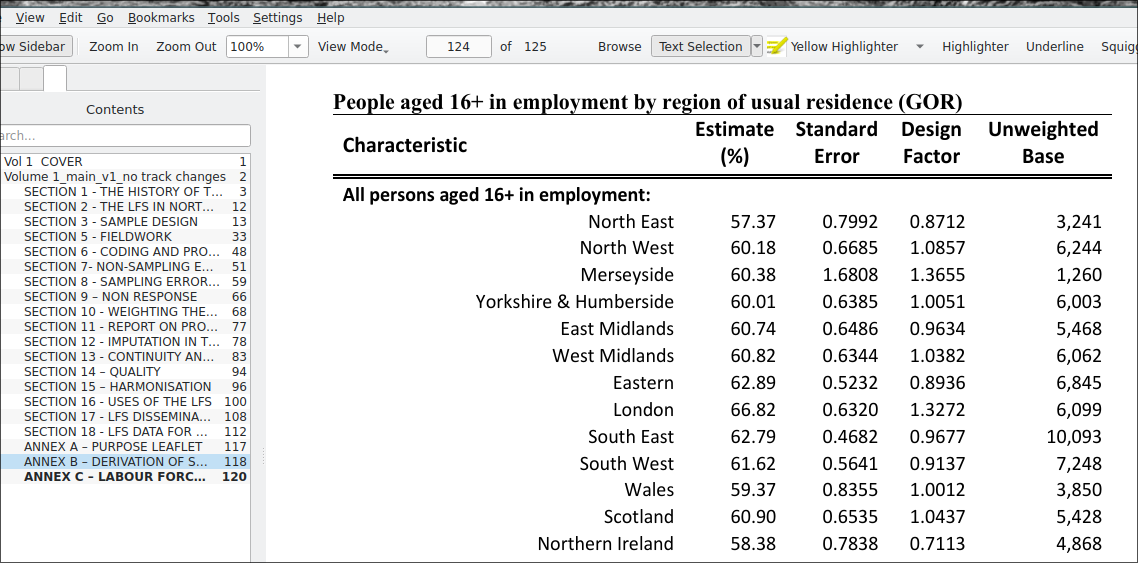
\includegraphics{pics/lfs_vol1_SE.pdf}

}

\caption{Test}

\end{figure}

We can see that for some reason, the number regions has been reduced
from the original 16 to 13. We therefore need to recode our original
variable.

\begin{Shaded}
\begin{Highlighting}[]
\NormalTok{lfs}\OtherTok{\textless{}{-}}\NormalTok{lfs}\SpecialCharTok{\%\textgreater{}\%}\FunctionTok{mutate}\NormalTok{(}\AttributeTok{uresmc.fn=}\FunctionTok{case\_when}\NormalTok{(}
\NormalTok{          lfs}\SpecialCharTok{$}\NormalTok{uresmc.f}\SpecialCharTok{==}\StringTok{"Tyne \& Wear"} \SpecialCharTok{|}\NormalTok{ lfs}\SpecialCharTok{$}\NormalTok{uresmc.f}\SpecialCharTok{==} \StringTok{"Rest of Northern region"}\SpecialCharTok{\textasciitilde{}}\StringTok{"North East"}\NormalTok{,}
\NormalTok{          lfs}\SpecialCharTok{$}\NormalTok{uresmc.f}\SpecialCharTok{==}\StringTok{"South Yorkshire"} \SpecialCharTok{|}\NormalTok{ lfs}\SpecialCharTok{$}\NormalTok{uresmc.f}\SpecialCharTok{==} \StringTok{"West Yorkshire"} \SpecialCharTok{|}\NormalTok{ lfs}\SpecialCharTok{$}\NormalTok{uresmc.f}\SpecialCharTok{==} \StringTok{"Rest of Yorks \& Humberside"} \SpecialCharTok{\textasciitilde{}}\StringTok{"Yorkshire \& Humberside"}\NormalTok{,}
\NormalTok{          lfs}\SpecialCharTok{$}\NormalTok{uresmc.f}\SpecialCharTok{==}\StringTok{"Inner London"} \SpecialCharTok{|}\NormalTok{ lfs}\SpecialCharTok{$}\NormalTok{uresmc.f}\SpecialCharTok{==} \StringTok{"Outer London"}\SpecialCharTok{\textasciitilde{}}\StringTok{"London"}\NormalTok{,}
\NormalTok{          lfs}\SpecialCharTok{$}\NormalTok{uresmc.f}\SpecialCharTok{==}\StringTok{"West Midlands (met county)"} \SpecialCharTok{|}\NormalTok{ lfs}\SpecialCharTok{$}\NormalTok{uresmc.f}\SpecialCharTok{==} \StringTok{"Rest of West Midlands"}\SpecialCharTok{\textasciitilde{}}\StringTok{"West Midlands"}\NormalTok{,}
\NormalTok{          lfs}\SpecialCharTok{$}\NormalTok{uresmc.f}\SpecialCharTok{==}\StringTok{"Greater Manchester"} \SpecialCharTok{|}\NormalTok{ lfs}\SpecialCharTok{$}\NormalTok{uresmc.f}\SpecialCharTok{==} \StringTok{"Rest of North West"}\SpecialCharTok{\textasciitilde{}}\StringTok{"North West"}\NormalTok{,}
\NormalTok{          lfs}\SpecialCharTok{$}\NormalTok{uresmc.f}\SpecialCharTok{==}\StringTok{"Strathclyde"} \SpecialCharTok{|}\NormalTok{ lfs}\SpecialCharTok{$}\NormalTok{uresmc.f}\SpecialCharTok{==} \StringTok{"Rest of Scotland"}\SpecialCharTok{\textasciitilde{}}\StringTok{"Scotland"}\NormalTok{,}
          \AttributeTok{.default=}\NormalTok{uresmc.f}
\NormalTok{          ))}
\end{Highlighting}
\end{Shaded}

For convenience, reorder the factor levels in order to match the ONS
ordering:

\begin{Shaded}
\begin{Highlighting}[]
\NormalTok{lfs}\SpecialCharTok{$}\NormalTok{uresmc.fn}\OtherTok{\textless{}{-}}\FunctionTok{as.factor}\NormalTok{(lfs}\SpecialCharTok{$}\NormalTok{uresmc.fn)}
\NormalTok{lfs}\SpecialCharTok{$}\NormalTok{uresmc.fn}\OtherTok{\textless{}{-}}\FunctionTok{factor}\NormalTok{(lfs}\SpecialCharTok{$}\NormalTok{uresmc.fn,}\AttributeTok{levels =} \FunctionTok{levels}\NormalTok{(lfs}\SpecialCharTok{$}\NormalTok{uresmc.fn)[}\FunctionTok{c}\NormalTok{(}\DecValTok{5}\NormalTok{,}\DecValTok{6}\NormalTok{,}\DecValTok{4}\NormalTok{,}\DecValTok{13}\NormalTok{,}\DecValTok{2}\NormalTok{,}\DecValTok{12}\NormalTok{,}\DecValTok{1}\NormalTok{,}\DecValTok{3}\NormalTok{,}\DecValTok{8}\NormalTok{,}\DecValTok{10}\NormalTok{,}\DecValTok{11}\NormalTok{,}\DecValTok{9}\NormalTok{,}\DecValTok{7}\NormalTok{)])}
\end{Highlighting}
\end{Shaded}

Let us now check the results:

\begin{Shaded}
\begin{Highlighting}[]
\NormalTok{lfs.s}\OtherTok{\textless{}{-}}\FunctionTok{svydesign}\NormalTok{(}\AttributeTok{ids=}\SpecialCharTok{\textasciitilde{}}\DecValTok{1}\NormalTok{,}\AttributeTok{weights=}\SpecialCharTok{\textasciitilde{}}\NormalTok{piwt22,}\AttributeTok{data=}\NormalTok{lfs}\SpecialCharTok{\%\textgreater{}\%}\FunctionTok{filter}\NormalTok{(ilodefr}\SpecialCharTok{==}\DecValTok{1}\NormalTok{)) }
\FunctionTok{round}\NormalTok{(}\FunctionTok{confint}\NormalTok{(}\FunctionTok{svytotal}\NormalTok{(}\SpecialCharTok{\textasciitilde{}}\NormalTok{uresmc.fn,lfs.s)))}
\end{Highlighting}
\end{Shaded}

\begin{verbatim}
                                  2.5 %  97.5 %
uresmc.fnNorth East             1108265 1366323
uresmc.fnNorth West             2056142 2462448
uresmc.fnMerseyside              473854  749424
uresmc.fnYorkshire & Humberside 2077728 2449422
uresmc.fnEast Midlands          1884931 2240257
uresmc.fnWest Midlands          2268450 2730368
uresmc.fnEast Anglia            1018147 1293525
uresmc.fnLondon                 3620425 4367581
uresmc.fnRest of South East     5133587 5816347
uresmc.fnSouth West             2150551 2532611
uresmc.fnWales                  1101246 1410746
uresmc.fnScotland               2178250 2671214
uresmc.fnNorthern Ireland        689076  803340
\end{verbatim}

We can now import the design factors from the LFS documentation. This
has to be done by hand, by directly copying the relevant numbers from
the lfs

While we are at it we can also improve the original table:

\begin{Shaded}
\begin{Highlighting}[]
\NormalTok{tot}\OtherTok{\textless{}{-}}\FunctionTok{data.frame}\NormalTok{(}\FunctionTok{svytotal}\NormalTok{(}\SpecialCharTok{\textasciitilde{}}\NormalTok{uresmc.fn,lfs.s))}
\NormalTok{tot}\SpecialCharTok{$}\NormalTok{deft}\OtherTok{\textless{}{-}}\FunctionTok{c}\NormalTok{(}\FloatTok{0.8712}\NormalTok{,}\FloatTok{1.0857}\NormalTok{,}\FloatTok{1.3655}\NormalTok{,}\FloatTok{1.0051}\NormalTok{,}\FloatTok{0.9634}\NormalTok{,}\FloatTok{1.0382}\NormalTok{,}\FloatTok{0.8936}\NormalTok{,}\FloatTok{1.3272}\NormalTok{,}\FloatTok{0.9677}\NormalTok{,}\FloatTok{0.9137}\NormalTok{,}\FloatTok{1.0012}\NormalTok{,}\FloatTok{1.0437}\NormalTok{,}\FloatTok{0.7113}\NormalTok{)}
\NormalTok{tot[}\StringTok{"2.5\%"}\NormalTok{]}\OtherTok{\textless{}{-}}\NormalTok{tot}\SpecialCharTok{$}\NormalTok{total}\SpecialCharTok{{-}}\NormalTok{(}\FloatTok{1.96}\SpecialCharTok{*}\NormalTok{tot}\SpecialCharTok{$}\NormalTok{SE}\SpecialCharTok{*}\NormalTok{tot}\SpecialCharTok{$}\NormalTok{deft)}
\NormalTok{tot[}\StringTok{"97.5\%"}\NormalTok{]}\OtherTok{\textless{}{-}}\NormalTok{tot}\SpecialCharTok{$}\NormalTok{total}\SpecialCharTok{+}\NormalTok{(}\FloatTok{1.96}\SpecialCharTok{*}\NormalTok{tot}\SpecialCharTok{$}\NormalTok{SE}\SpecialCharTok{*}\NormalTok{tot}\SpecialCharTok{$}\NormalTok{deft)}
\FunctionTok{rownames}\NormalTok{(tot)}\OtherTok{\textless{}{-}}\FunctionTok{substr}\NormalTok{(}\FunctionTok{rownames}\NormalTok{(tot),}\DecValTok{10}\NormalTok{,}\FunctionTok{nchar}\NormalTok{(}\FunctionTok{rownames}\NormalTok{(tot)))}
\FunctionTok{kable}\NormalTok{(}\FunctionTok{round}\NormalTok{(tot[,}\FunctionTok{c}\NormalTok{(}\StringTok{"2.5\%"}\NormalTok{,}\StringTok{"97.5\%"}\NormalTok{)]))}
\end{Highlighting}
\end{Shaded}

\begin{tabular}{l|r|r}
\hline
  & 2.5\% & 97.5\%\\
\hline
North East & 1124882 & 1349706\\
\hline
North West & 2038728 & 2479862\\
\hline
Merseyside & 423490 & 799788\\
\hline
Yorkshire \& Humberside & 2076776 & 2450374\\
\hline
East Midlands & 1891430 & 2233758\\
\hline
West Midlands & 2259623 & 2739195\\
\hline
East Anglia & 1032794 & 1278878\\
\hline
London & 3498181 & 4489825\\
\hline
Rest of South East & 5144607 & 5805327\\
\hline
South West & 2167034 & 2516128\\
\hline
Wales & 1101057 & 1410935\\
\hline
Scotland & 2167474 & 2681990\\
\hline
Northern Ireland & 705569 & 786847\\
\hline
\end{tabular}

\hypertarget{answers}{%
\subsubsection{Answers}\label{answers}}

\textbf{Question 1} The 2017 BSA is a three stage stratified random
survey, with postcode sectors, adresses and individuals as the units
selected at each stage. Primary sampling units were stratified according
to geographies (sub regions), population density, and proportion of
owner-occupiers. Sampling rate was proportional to the size of postcode
sectors (ie number of addresses).

\textbf{Question 2} From the Data Dictionary it appears that the primary
sampling units (sub regions) are identified by \texttt{Spoint} and the
strata by \texttt{StratID}. The weights variable is \texttt{WtFactor}.
Addresses are not provided but could be approximated with a household
identifier.

\textbf{Question 3} Not using weights would make us overestimate the
mean age in the population (of those aged 16+) by about 4 years. This is
likely to be due to the fact that older respondents are more likely to
take part to surveys. Using survey design variables does not alter the
value of the estimated population mean. However, not accounting for it
would lead us to overestimate the precision/underestimate the
uncertainty of our estimate with a narrower confidence interval -- by
about plus or minus 3 months.

\textbf{Question 4} The proportion of 17-34 year old in the sample is
28.5 and its 95\% confidence interval 26.5, 30.6

\textbf{Question 5} The 95\% confidence interval for the proportion of
people interested in politics in the South West is 39.8-53.4. By
contrast, it is 47.6-60.8 in London. The region with the lowest
precision of estimates (ie the widest confidence interval) is Wales,
with a 20 percentage point difference between the upper and lower bounds
of the confidence interval.

\textbf{Question 6}

\begin{verbatim}
             I(Politics.s == "Significantly") ci_l ci_u
17-34.Male                               42.9 37.7 48.2
35-54.Male                               50.8 46.6 54.9
55+.Male                                 57.8 53.9 61.6
17-34.Female                             26.3 22.0 31.1
35-54.Female                             34.1 30.6 37.8
55+.Female                               43.0 39.6 46.5
\end{verbatim}

Older respondents both male and female tend to be more involved in
politics than younger ones.

The confidence interval for the proportion of men under 35 and women
above 55 interested in politics overlaps; it is unlikely that they
differ in the population.

\hypertarget{spss-examples}{%
\section{6. SPSS Examples}\label{spss-examples}}

At the time of writing this document (September 2023) Standard editions
of SPSS did not include support for estimation with survey design
variables, and only limited use of sampling weights. When using grossing
weights -- ie weight that have been designed to enable computing
population totals from sample data -- as is the case for instance with
the Labour Force and Family Resources surveys, measures of dispersion
and standard errors will not be adequately computed. It is therefore not
recommended to attempt using the base version of SPSS with survey data
beyond estimating point estimates. Significance testing, and standard
errors will not reflect the correct values. Users willing to use SPSS
with survey data will need to acquire the Premium Edition or the Complex
Samples add-on of the software.

In this exercise, we will practice statistical inference with data from
the
\href{https://beta.ukdataservice.ac.uk/datacatalogue/studies/study?id=8450}{2017
British Social Attitudes Survey (BSA)} taking into account weights and
survey design variables. Please note that at the time of writing this
document only some of the BSA editions include survey design variables.

\hypertarget{identifying-the-survey-design-and-variables-1}{%
\subsection{6.1 Identifying the survey design and
variables}\label{identifying-the-survey-design-and-variables-1}}

We first need to find out about the survey design that was used in the
2017 BSA, and the design variables that are made available in the
dataset. Such information can usually be found in the documentation that
comes together with the data under the \texttt{mrdoc/pdf} folder.

\textbf{Question 1} What is the design that was used in this survey (ie
how many stages were there, and what were the units sampled). What were
the primary sampling units; the strata (if relevant)?

Now that we are a bit more familiar with the way the survey was
designed, we need to try and identify the design variables we can
include when producing estimates. The information can usually be found
in the user manual or the data dictionary available under
\texttt{mrdoc/ukda\_data\_dictionaries.zip} You may need to decompress
the file separately

\textbf{Question 2} What survey design variables are available? Are
there any ones that are missing -- if so which ones? What is the name of
the weights variables?

\hypertarget{specifying-the-survey-design-1}{%
\subsection{6.2 Specifying the survey
design}\label{specifying-the-survey-design-1}}

Let us first open the 2017 BSA dataset.

\begin{verbatim}
CD 'C:\Users\mscsepw2\OneDrive - The University of Manchester\Surveyskills'.
  GET 
    FILE=' BSA\UKDA-8450-spss\spss\spss25\bsa2017_for_ukda.sav'.
\end{verbatim}

In principle, we should tell SPSS that we are working with a three stage
stratified cluster sample. In practice however, we only have information
about the initial ie primary sampling units.\\
This is achieved with the \texttt{CSPLAN} command through we create a
plan file which contains the survey design information.

\begin{verbatim}
CSPLAN ANALYSIS
  /PLAN FILE='bsa17_SPSS_design.csaplan'
  /PLANVARS ANALYSISWEIGHT=WtFactor       
  /SRSESTIMATOR TYPE=WOR
  /PRINT PLAN
  /DESIGN STAGELABEL='S1' STRATA=StratID CLUSTER=Spoint 
  /ESTIMATOR TYPE=WR.
\end{verbatim}

\hypertarget{mean-age-and-its-95-confidence-interval-1}{%
\subsection{6.3 Mean age and its 95\% confidence
interval}\label{mean-age-and-its-95-confidence-interval-1}}

We can now produce a first set of estimates using this design and
compare them with those we would have got without accounting for it. We
will compute the average (ie mean) age of respondents in the sample, as
well as the proportion of male and female respondents aged over 55. We
will need to use \texttt{/CSDESCRIPTIVES}

\begin{verbatim}
DATASET ACTIVATE DataSet1.
* Complex Samples Descriptives.
CSDESCRIPTIVES
  /PLAN FILE='bsa17_SPSS_design.csaplan'
  /SUMMARY VARIABLES=RAgeE
  /MEAN
  /STATISTICS SE CIN(95)
  /MISSING SCOPE=ANALYSIS CLASSMISSING=EXCLUDE.
\end{verbatim}

Under the \texttt{/STATISTICS} command we can request either or both the
standard error of the mean and its 95\% confidence interval.

What difference would it make to the estimates and 95\% CI to compute
respectively, an unweighted mean, as well as a weighted mean without
accounting for the survey design?

\textbf{Unweighted means and CI}

\begin{verbatim}
DESCRIPTIVES VARIABLES=RAgeE
  /STATISTICS=MEAN SEMEAN.
\end{verbatim}

SPSS does not provide an option for computing confidence intervals in
this case, but we know that a 95\% confidence interval is the sample
mean respectively minus and plus 1.96 times its standard error. Using
the SPSS output, we can compute it ourselves as 1.96*.2872=about .56
years, that is close to 7 months.

\textbf{Weighted means and CI without survey design}

\begin{verbatim}
WEIGHT BY WtFactor.
DESCRIPTIVES VARIABLES=RAgeE
  /STATISTICS=MEAN SEMEAN.
WEIGHT OFF.
\end{verbatim}

\textbf{Question 3} What would be the consequences of weighing but not
accounting for the sample design; not using weights and accounting for
the sample design when:

\begin{itemize}
\tightlist
\item
  inferring the mean value of the population age?
\item
  inferring the uncertainty of our estimate of the population age?
\end{itemize}

\hypertarget{computing-a-proportion-and-its-95-confidence-interval-1}{%
\subsection{6.4 Computing a proportion and its 95\% confidence
interval}\label{computing-a-proportion-and-its-95-confidence-interval-1}}

We can now similarly compute an estimate of a proportion (or percentage)
of a categorical variable in the population. For instance, the
proportion of people who declare themselves interested in politics. This
is the \texttt{Politics} variable. It has five categories that we are
going to recode into `Significantly' (interested) and `Not'
(significantly) in order to simplify the analysis.

\begin{verbatim}
FREQUENCIES VARIABLES=Politics
  /ORDER=ANALYSIS.

RECODE Politics (9=SYSMIS) (1 thru 2=1) (3 thru 5=2) INTO Politics.s.
EXECUTE.

VARIABLE LABELS
Politics.s   "Whether significantly interested in politics".
VALUE LABELS
Politics.s
1  "Significant"
2  "Not significant". 
EXECUTE.

FREQUENCIES VARIABLES=Politics.s
  /ORDER=ANALYSIS.

WEIGHT BY WtFactor.
FREQUENCIES VARIABLES=Politics.s
  /ORDER=ANALYSIS.
WEIGHT OFF.
\end{verbatim}

As with the mean of age earlier, we can see that the weighted and
unweighted point estimates of the proportion of respondents
significantly interested in politics change, even if slightly, and that
they remain the same when survey design is accounted for.

With the help of \texttt{CSTABULATE} we can examine frequencies,
proportions and confidence intervals of these proportions accounting for
the survey design. As before, the point estimates do not further change
once survey design is accounted for.

\begin{verbatim}
* Complex Samples Frequencies.
CSTABULATE
  /PLAN FILE='bsa17_SPSS_design.csaplan'
  /TABLES VARIABLES=Politics.s
  /CELLS POPSIZE TABLEPCT
  /STATISTICS CIN(95) 
  /MISSING SCOPE=TABLE CLASSMISSING=EXCLUDE.
\end{verbatim}

\textbf{Question 4} What is the proportion of respondents aged 17-34 in
the sample, as well as its 95\% confidence interval? You can use
\texttt{RAgecat5}

\hypertarget{domain-ie-subpopulation-estimates}{%
\subsection{6.5 Domain (ie subpopulation)
estimates}\label{domain-ie-subpopulation-estimates}}

Although computing estimates for specific groups (for example the
average age of people who report being interested in politics) is not
conceptually different from doing it for the sample as a whole, doing it
with weights as part of an inferential analysis requires some caution.
Calculating weighted estimates for a subpopulation while the rest of the
sample is left out of the analysis might yield incorrect results. This
is why using survey design informed functions is particularly
recommended when doing such analyses.

The SPSS command \texttt{CSDESCRIPTIVES} that we used above makes such
domain estimation relatively straightforward. If we would like to
compute the mean age of BSA respondents by government office regions, we
need to specify:

\begin{itemize}
\tightlist
\item
  The outcome variable whose estimate we want to compute: ie
  \texttt{RAgeE}
\item
  The grouping variable(s) \texttt{GOR\_ID}
\item
  And the type of type of variance estimation we would like to see
  displayed ie standard errors or confidence interval
\end{itemize}

\begin{verbatim}
 * Complex Samples Descriptives.
CSDESCRIPTIVES
  /PLAN FILE='bsa17_SPSS_design.csaplan'
  /SUMMARY VARIABLES=RAgeE
  /SUBPOP TABLE=GOR_ID DISPLAY=LAYERED
  /MEAN
  /STATISTICS CIN(95)
  /MISSING SCOPE=ANALYSIS CLASSMISSING=EXCLUDE.
\end{verbatim}

Our inference seem to suggest that the population in London is among the
youngest in the country, and that those in the South West are among the
oldest -- their respective 95\% confidence intervals do not overlap. We
should not feel so confident about differences between London and the
South East for example, as the CIs partially overlap.

We can also examine proportions for subpopulations. In order to do this,
we need to specify the category of the variable we are interested in as
an outcome.For instance, the syntax below uses respondents who are
significantly interested in politics:

\begin{verbatim}
* Complex Samples Frequencies.
CSTABULATE
  /PLAN FILE='bsa17_SPSS_design.csaplan'
  /TABLES VARIABLES=Politics.s
  /SUBPOP TABLE=GOR_ID DISPLAY=LAYERED
  /CELLS TABLEPCT
  /STATISTICS CIN(95) 
  /MISSING SCOPE=TABLE CLASSMISSING=EXCLUDE.
\end{verbatim}

\textbf{Question 5} What is the 95\% confidence interval for the
proportion of people interested in politics in the South West? Is the
proportion likely to be different in London? In what way? What is the
region of the UK for which the precision of the estimates is likely to
be the smallest?

When using \texttt{CSTABULATE}, we can define domains or subpopulations
with several variables, not just one. For example, we could look at
gender differences in political affiliations by regions. However, as the
size of subgroups decrease, so does the precision of the estimates as
their confidence interval widens, to a point where their substantive
interest is not meaningful anymore.

\textbf{Question 6} Using interest in politics as before, and three
category age \texttt{RAgecat5}:

\begin{itemize}
\item
  Produce a table of results showing the proportion of respondents
  significantly interested in Politics by age group and gender
\item
  Assess whether the age difference in interest for politics is similar
  for each gender?
\item
  Based on the data, is it fair to say that men aged under 35 tend to be
  more likely to declare themselves interested in politics than women
  aged 55 and above?
\end{itemize}

\begin{verbatim}
CSTABULATE
  /PLAN FILE='bsa17_SPSS_design.csaplan'
  /TABLES VARIABLES=Politics.s
  /SUBPOP TABLE=Rsex BY RAgecat5 DISPLAY=LAYERED
  /CELLS TABLEPCT
  /STATISTICS CIN(95) 
  /MISSING SCOPE=TABLE CLASSMISSING=EXCLUDE.
\end{verbatim}

\hypertarget{answers-1}{%
\subsubsection{Answers}\label{answers-1}}

\textbf{Question 1} The 2017 BSA is a three stage stratified random
survey, with postcode sectors, adresses and individuals as the units
selected at each stage. Primary sampling units were stratified according
to geographies (sub regions), population density, and proportion of
owner-occupiers. Sampling rate was proportional to the size of postcode
sectors (ie number of addresses).

\textbf{Question 2} From the Data Dictionary it appears that the primary
sampling units (sub regions) are identified by \texttt{Spoint} and the
strata by \texttt{StratID}. The weights variable is \texttt{WtFactor}.
Addresses are not provided but could be approximated with a household
identifier.

\textbf{Question 3} Not using weights would make us overestimate the
mean age in the population (of those aged 16+) by about 4 years. This is
likely to be due to the fact that older respondents are more likely to
take part to surveys. Using survey design variables does not alter the
value of the estimated population mean. However, not accounting for it
would lead us to overestimate the precision/underestimate the
uncertainty of our estimate with a narrower confidence interval -- by
about plus or minus 3 months.

\textbf{Question 4} The proportion of 17-34 year old in the sample is
28.5 and its 95\% confidence interval 26.5, 30.6

\textbf{Question 5} The 95\% confidence interval for the proportion of
people interested in politics in the South West is 39.8-53.4. By
contrast, it is 47.6-60.8 in London. The region with the lowest
precision of estimates (ie the widest confidence interval) is Wales,
with a 20 percentage point difference between the upper and lower bounds
of the confidence interval.

\textbf{Question 6}

\begin{verbatim}
             I(Politics.s == "Significantly") ci_l ci_u
17-34.Male                               42.9 37.7 48.2
35-54.Male                               50.8 46.6 54.9
55+.Male                                 57.8 53.9 61.6
17-34.Female                             26.3 22.0 31.1
35-54.Female                             34.1 30.6 37.8
55+.Female                               43.0 39.6 46.5
\end{verbatim}

Older respondents both male and female tend to be more involved in
politics than younger ones.

The confidence interval for the proportion of men under 35 and women
above 55 interested in politics overlaps; it is unlikely that they
differ in the population.

\hypertarget{stata-examples}{%
\section{7 Stata examples}\label{stata-examples}}

Stata provides comprehensive support for computing estimates from survey
data. Users may either opt to add sampling weights to the standard
estimation commands, or use survey-specific commands. The latter is
recommended when knowledge of estimate precision is required. Stata
provides a conceptual distinction between four types of weights:

\begin{itemize}
\tightlist
\item
  frequency weights (\texttt{fweight}),
\item
  analytical weights (\texttt{aweight}),
\item
  importance weights (\texttt{iweight}) and
\item
  probability weights (\texttt{pweight}).
\end{itemize}

These differences impact on the way standard errors are computed during
estimation. In most cases, social survey weights from UKDS datasets
should be treated as probability weights. A number of of basic
estimation commands, such as \emph{summarise} do not allow using
probability weights. This is an explicit features of Stata, meant to
nudge users of survey data to prioritise the survey commands rather than
`casual' weighting.

Using standalone weight specification (ie not using survey design
functions). In Stata it consists in the weighting variable being
specified between square brackets. Stata defines four kind of weights:

Only probability weights (abbreviated as \texttt{pw} in most Stata
commands) should be used with survey data. However, Stata does not allow
using them with its main commands, for the reason highlighted above ie
in order for users not overlook survey design issues in their data.
Therefore, one has to specify instead the wrong frequency weights
(\texttt{fw}) if one does not wish to use the survey design functions.

\hypertarget{appendix-study-specific-weighting-and-sample-design-information}{%
\section{8. Appendix: Study-specific weighting and sample design
information}\label{appendix-study-specific-weighting-and-sample-design-information}}

\hypertarget{british-social-attitudes-survey}{%
\subsection{8.1 British Social Attitudes
Survey}\label{british-social-attitudes-survey}}

The BSA is a three stage stratified random survey, with postcode
sectors, addresses and individuals as the units selected at each stage.
Primary sampling units were furthermore stratified according to
geographies (sub regions), population density, and proportion of
owner-occupiers. Sampling rate was proportional to the size of postcode
sectors (ie number of addresses). Some issues of the BSA such as the
2017 include survey design information. The 2017 issue included
information about Primary Smapling Units (\texttt{Spoint}), strata
(\texttt{StratID}). Weights are called \texttt{WtFactor}.

\hypertarget{labour-force-survey}{%
\subsection{8.2 Labour Force Survey}\label{labour-force-survey}}

The LFS is a geographically stratified random survey. For the main part
Primary sampling units are addresses within postcode sectors, drawn from
the Small Users Postcode Address File (PAF). The small users PAF is
limited to addresses which receive, fewer than 50 items of post per day.
In a small number of cases a second stage sampling occurs where several
households exist at a given address. A clustering effect is also present
to the extent that units of observations are individuals withing
households, and that some groups are clustered within these, typically
ethnicity. LFS weights: - PWTxx -- person level sampling weight; enables
inferring population counts - IWTxx - Person-level sampling weight for
income analysis (ie subsample of people in paid work) - PHHWTxx -
Household-level sampling weight (for household-level analysis)

\hypertarget{family-resources-survey}{%
\subsection{8.3 Family Resources Survey}\label{family-resources-survey}}

The FRS is a stratified clustered random survey, with survey design
differing slightly between countries of the UK. In Great Britain,
Primary sampling units are postcode sectors, drawn from the Small Users
Postcode Address File (PAF). Before being selected, PSUs are stratified
according to geography, proportion of household reference persons from
higher social classes in the area, proportion of economically active
respondents in the area, and proportion of economically active men who
ware unemployed. In Northern Ireland, the sample is a systematic random
sample of addresses.

Information about Design Effect in the Family Resources Survey series is
available
\href{https://assets.publishing.service.gov.uk/government/uploads/system/uploads/attachment_data/file/972808/Ch1_Methodology_and_Standard_Errors.xlsx}{here}

FRS weights: GROSS4: person-level sampling weight; enables inferring
population counts

\hypertarget{references}{%
\section{9. References}\label{references}}

(\textbf{PierreWal?}) : and here

\hypertarget{refs}{}
\begin{CSLReferences}{1}{0}
\leavevmode\vadjust pre{\hypertarget{ref-Blair2014}{}}%
Blair, Johnny. 2014. \emph{Designing Surveys : A Guide to Decisions and
Procedures.} 3rd edition / Johnny Blair, Ronald F. Czaja, Edward A.
Blair. Los Angeles: SAGE.

\leavevmode\vadjust pre{\hypertarget{ref-DWP2014}{}}%
DWP. 2014. {``Uncertainty in Family Resources Survey-Based Analysis.
Guidance on Estimating Uncertainty in Family Resources Survey-Based
Analysis.''} Edited by Department for Work and Pensions. 2014.
\url{https://www.gov.uk/government/publications/uncertainty-in-family-resources-survey-based-analysis}.

\leavevmode\vadjust pre{\hypertarget{ref-IBM2020}{}}%
IBM Support. 2020. {``Inconsistency in the Output When Using Weighting
Procedure. IBM Support Document Number 419449.''} 2020.
\url{https://www.ibm.com/support/pages/inconsistency-output-when-using-weighting-procedure}.

\leavevmode\vadjust pre{\hypertarget{ref-Kish1995}{}}%
Kish, Leslie. 1995. \emph{Survey Sampling}. Wiley Classics Library. New
York: Wiley.

\leavevmode\vadjust pre{\hypertarget{ref-Lohr20192010}{}}%
Lohr, Sharon L. 2019 - 2010. \emph{Sampling : Design and Analysis}.
Second edition. Texts in Statistical Science. Boca Raton, FL: CRC Press.

\leavevmode\vadjust pre{\hypertarget{ref-Lumley2023}{}}%
Lumley, Thomas. 2023. {``Survey: Analysis of Complex Survey Samples.''}

\leavevmode\vadjust pre{\hypertarget{ref-ONS2022}{}}%
ONS. 2022. {``Family Resources Survey, 2020/21 Methodology and Standard
Error Tables.''} Edited by Office for National Statistics. 2022.
\url{https://assets.publishing.service.gov.uk/government/uploads/system/uploads/attachment_data/file/1065513/Ch1_Methodology_and_Standard_Errors.ods}.

\leavevmode\vadjust pre{\hypertarget{ref-Curran2016}{}}%
P, Curran. 2016. {``Complex Survey Designs and Weighting Using Stata:
Part 1-3.''} 2016. \url{https://www.youtube.com/watch?v=oOpJdC_oeKY}.

\leavevmode\vadjust pre{\hypertarget{ref-UKDS2018}{}}%
UKDS. 2018. {``Data Skills Modules: Applying Weights to Survey Data.''}
Edited by UK Data Service. 2018.
\url{https://www.youtube.com/watch?v=TIad5__WP8g}.

\leavevmode\vadjust pre{\hypertarget{ref-UKDS2019}{}}%
---------. 2019. {``Weights in Social Surveys: An Introduction:''}
Edited by UK Data Service. 2019.
\url{https://www.youtube.com/watch?v=Vllr4olp3N4\&t=39s}.

\leavevmode\vadjust pre{\hypertarget{ref-Wallrich2019}{}}%
Wallrich, Lukas. 2019. {``Week 7 Using Survey Weights in r.''} Edited by
Goldsmiths Core Quantitative Methods Series. 2019.
\url{https://www.youtube.com/watch?v=brxx81U6N1o}.

\end{CSLReferences}



\end{document}
